\chapter{Astrophysics around neutron stars}
\chapterimage[width=15cm]{wordcloud/chap3b.png}

Let us now discuss the violent environments around neutron stars and the related astrophysics therein.
These surroundings play an important role when we try to decipher the observations of these stars.

Typically, the neutron stars can be found (or rather seen) either in binary systems where they are accompanied by another star, or as a lonely remnant left behind from a supernova explosion.
In the latter case it is the neutron star itself that is the source of the energy that renders it visible as it will slowly cool down and radiate away all the left-over heat from the explosion.
In some cases, the rotating magnetic field of the star can also create radiation when it propels in the medium that is left behind.
This gives rise to a particle acceleration as the charged plasma is dragged along by the magnetic field producing radiation as the particles try to resist this motion.

In the binary systems, on the other hand, the energy originates not from the neutron star itself but from the companion.
In the heart of this whole problem is an astrophysical process called accretion.
This is a physical process where matter is transferred from one source to another because of the gravitational forces.
In the following discussion we will focus on these binary systems and on the so-called accretion powered phenomena.

%In this thesis, we will focus on extracting the information from the so-called X-ray bursts that ignite in the upper layers of neutron stars.
%These bursts originate from the unstable nuclear fusion runaways in the neutron star ocean that produce excessive heat that is then radiated away as photons.
%These photons will then emerge through the atmosphere of the star, travel astronomical distances towards Earth until they will land on one of our scientific instruments, and be recorded by us as X-ray events.
%In theory, this method of using the X-ray bursts to probe the neutron star interiors is robust as we can theoretically model the characteristics of the emerging radiation and these models can be applied to describe the data that we see. 
%In practice, however, caution is needed when applying the models as the environment near the neutron star plays a huge role.


In this final chapter, we will shortly discuss the complex astrophysical environment surrounding the bursting neutron star.
We will also review the relevant physics behind the X-ray bursts.


%\section{Astrophysics around neutron stars}
%Let us begin by discussing the violent environments around the neutron stars as the these surroundings play an important role when we try to decipher the real observations of these stars.
 
%Typically, the neutron stars can be found (or rather seen) either in binary systems where they are accompanied by another star, or as a lonely remnant left behind from a supernova explosion.
%In the latter case it is the neutron star itself that is the source of the energy that renders it visible as it will slowly cool down and radiate away all the left-over heat from the explosion.
%In some cases, the rotating magnetic field of the star can also create radiation when it propels in the medium that is left behind.
%This gives rise to a particle acceleration as the charged plasma is dragged along by the magnetic field producing radiation as the particles try to resist this motion.
 
 
%In the binary systems, on the other hand, the energy originates not from the neutron star itself but from the companion.
%In the heart of this whole problem is an astrophysical process called accretion.
%This is a physical process where matter is transferred from one source to another because of the gravitational forces.
%In this thesis and in the following discussion we will focus on these binary systems and on the so-called accretion powered phenomena.

%We, however, note that it is possible to use the observations of the single neutron star remnants too, to constrain the mass and radius.\cite[see, e.g.,][]{PR06}



\section{Accretion}

Accretion is an astrophysical process that taps into the gravitational potential energy of particles.
It can be a source of enormous amounts of energy if the central object is compact, because the depth of a gravitational well is directly proportional to the compactness of the source.
Hence, it is an important, and often dominating, process for neutron stars.\cite[For an introduction, see e.g., ][]{FKR02}

Gravitational potential energy release for a mass $m$ that is accreted onto a compact object of radius $R$ and mass $M$ is
\be
\Delta E_{\mathrm{acc}} = m \frac{G M}{R} \sim 10^{20} \left( \frac{m}{\g} \right) \left( \frac{10\km}{R} \right) \left( \frac{M}{\Msun} \right) \erg,
\ee
where in the latter expression typical dimensions of neutron star are inserted to the formula.

This energy, $10^{20} \erg$ per each gram that is accreted, is usually released as radiation.
The rate of this energy release is simply related to the mass accreted per time, i.e., accretion rate $\Mdot$, 
\be
L_{\mathrm{acc}} = \Mdot \frac{G M}{R} \approx \Ten{1.3}{36} \left( \frac{\Mdot}{10^{16} \g\unitspace\mathrm{s}^{-1}} \right) \left( \frac{10\km}{R} \right) \left( \frac{M}{\Msun} \right) \ergs,
\ee
where a typical value of $\Mdot \sim 10^{16} \g\unitspace\mathrm{s}^{-1} \approx \Ten{1.5}{-10} \Msun\unitspace\mathrm{yr}^{-1}$ is taken for the accretion rate.
Hence, depending on the accretion rate, this value can be about the same as the Eddington luminosity \red{Eq. XXX} of a neutron star.

\red{X-rays from blackbody $T$}


\subsection{Roche lobes and mass transfer in binary systems}

In order to use the accretion as an energy source, we need mass transfer to occur.
For the mass transfer to keep on operating, a source of fresh material is needed.
In binary systems, the companions star is the obvious fuel resource.
Here we will focus on the so-called Low Mass X-ray Binary (LMXB) systems where the companion, like the name implies, is a relatively low-weight star.\cite{TH06}
Typically, it is a normal or late-type star with a mass $M \lesssim 1 \Msun$.
Such a setup leads to a mass-transfer quite naturally as the more heavy-weight neutron star will just rip out the outer layers of its poor companion and slowly devours it, until nothing is left.
As another option, the system could be a so-called High Mass X-ray Binary (HMXB) system, where the neutron star companion is $M \sim 10\Msun$, and the accretion happens, for example, via a neutron star traveling through the other stars extended outer envelope.
Here, we will, however, only focus on the LMXB systems, as they provide a relatively stable mass-transfer mechanism.


%Roche Lobe \cite{PRP02} \cite{LL15}
How exactly is the material transferred form the companion to the primary star is an interesting problem.
We can begin to understand the physical setup by considering a general hydrodynamical system of two objects in a rotating frame.
Here we select the frame such that it co-rotates with the binary system. % with an angular velocity $\omega$.
The subsequent flow of gas between the two stars can then be described by the Euler equation with additional Corriolis and XXX terms.\cite[see, e.g,][for a good introduction]{Cho98}
In practice the Euler equation describes the time evolution of the velocity $\vec{v}$ of the gas that has a pressure $P$ and density $\rho$.
In a reference frame rotating together with the binary system with angular velocity $\omega$ the Euler equation takes the form 
\be
\frac{ \partial \vec{v} }{\partial t} + (\vec{v} \cdot \nabla)\vec{v} = -\nabla \Phi_{\mathrm{R}} - 2 \vec{ \omega } \times \vec{v} - \frac{1}{\rho} \nabla P,
\ee
where the angular velocity of the binary is
\be
\vec{ \omega } = \left( \frac{ G M }{a^3} \right)^{1/2} \vec{e},
\ee
as given with the unit vector $\vec{e}$ normal to the orbital plane.
Here $M$ is the total mass of the system, i.e., $M = M_1 + M_2$, where $M_1$ and $M_2$ are the individual masses of the two stars in the system, respectively, and $a$ is their orbital separation.

\begin{figure}[t!]
%\centering
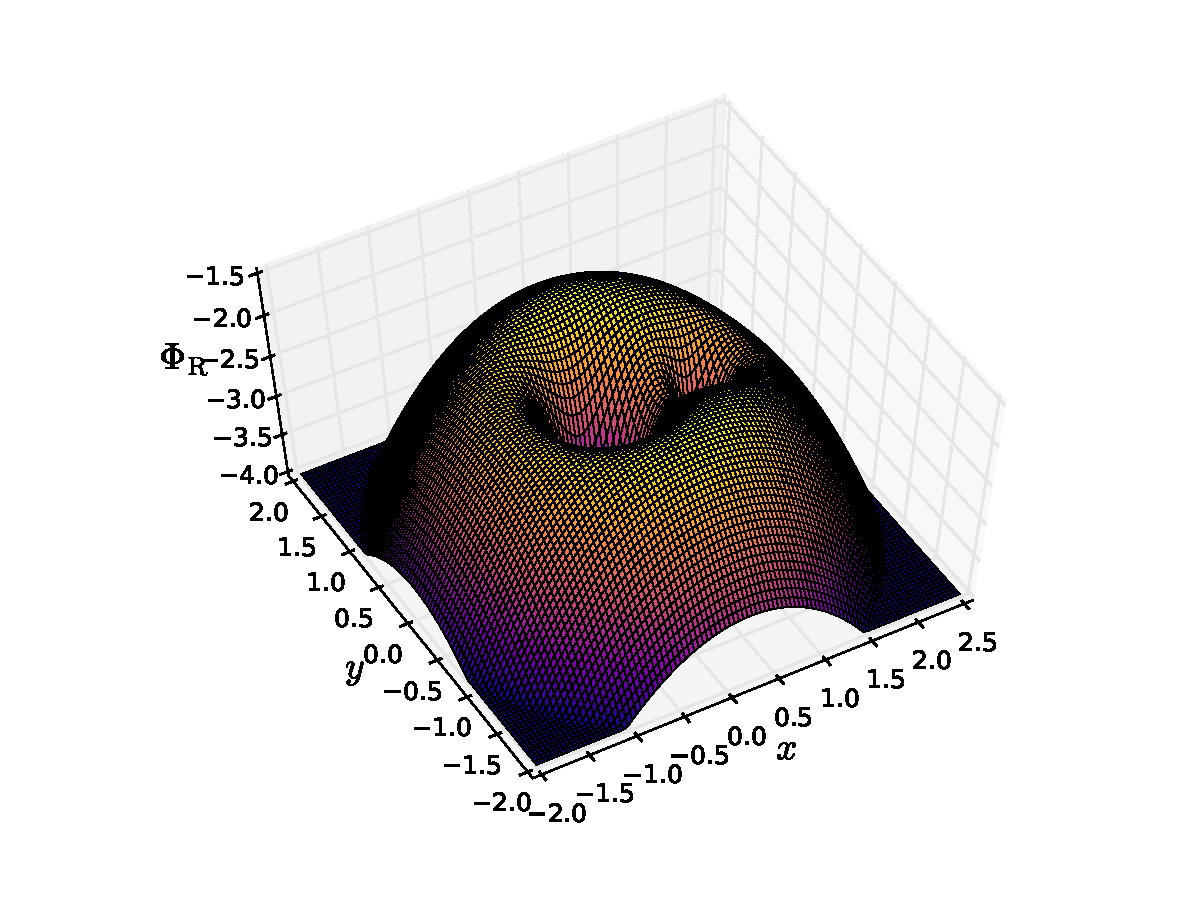
\includegraphics[width=16cm]{figs/astro/roche.pdf}
%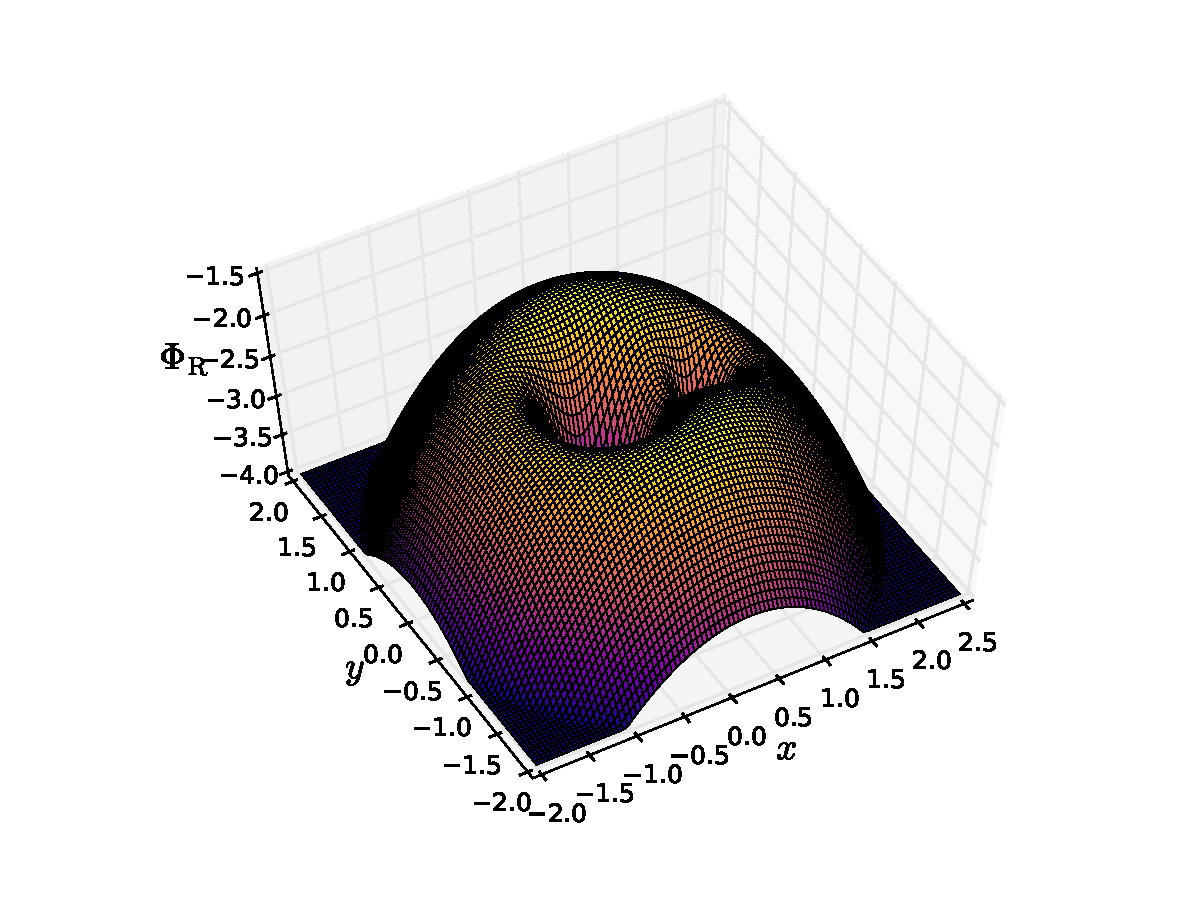
\includegraphics[width=7.5cm]{figs/astro/roche.pdf}
\caption{\label{fig:roche}
    Two-dimensional Roche potential $\Phi_{\mathrm{R}}(x,y)$ visualized for a binary systems with $M_1/M_2 = $ and $a = $.The nozzle ($L_1$ point) is visible as a valley (or more specifically, a saddle point) between the gravitational wells of the two stars.
}
\end{figure}

The effects originating from the gravitation and from the centrifugal forces are encapsulated in the so-called Roche potential, given as a function of radial vector $\vec{r}$ as\cite[see, e.g.,][]{PRP02, LL15}
\be
\Phi_{\mathrm{R}}(\vec{r}) = -\frac{G M_1}{|\vec{r} - \vec{r_1}|} -\frac{G M_2}{|\vec{r} - \vec{r_2}|} - \frac{1}{2} ( \vec{ \omega } \times \vec{v} )^2,
\ee
where the location of the stars are given with $\vec{r_1}$ and $\vec{r_2}$.
By studying the shape of the potential, we see that in between the stars, in the so-called $L_1$ point there exists a location where the countering gravitational forces from the two stars are balanced.
This can be though of as a physical nozzle in the system from which the less massive star will leak into the more massive star.
Such a mass transfer, also known as a Roche lobe overflow, will then occur if the companion star's radius exceeds the size of its own individual Roche lobe visualized in \fig{fig:roche}.
Typically such a thing can happen when the star evolves and expands at the end of its life cycle. 


\subsection{Accretion disks}

When the mass transfer has started via the Roche lobe overflow, and we have a stable source of material which transfers matter from the companion to the more massive neutron star, we can next focus on the region where gravitational forces of the neutron star dominate.
Most importantly, the infalling material has to somehow loose its angular momentum, before it is able to travel all the way to the neutron star surface.
Nature's mechanism to do this is called an accretion disk.

%accretion disk: machine for slowly lowering material in the graviational potential and extracting energy.
%orbital kinetic energy to heat

The must flow will be confined into the orbital plane of the binary system, hence, the problem is two dimensional as a first approximation.
This is known as the so-called thin-disk approximation because we neglect all the structure that the disk might have in the vertical direction.
Radial structure of the disk can be obtained from the Keplerian rotation law as
\be
\Omega_{\mathrm{K}}(R) = \left( \frac{G M }{R^3} \right)^{1/2},
\ee
describing an angular velocity as a function of radial coordinate from the disk center.

There is an important detail hidden here in the Kepler's law:
Keplerian angular velocity implies differential rotation, i.e., varying angular velocities as a function of the distance from the center of the disk.
Such a shearing between two adjacent annulus will then lead to viscous stresses when the inner annulus rotates faster than the outer one.

The disk's structure can be obtained from the hydrodynamical equations in cylindrical coordinates.
Instead of the density $\rho$, let us use the surface density $\Sigma = \rho H$ to describe the mass, where $H$ is the height of the disk.
Conservation of mass and angular momentum can then be written as\cite[see e.g.,][for full derivation]{Cho98, FKR02}
\be
r \frac{\partial \Sigma}{\partial t} + \frac{\partial}{\partial r}(r \Sigma v_r) = 0,
\ee
and
\be
r \frac{\partial}{\partial t}(\Sigma r^2 \Omega) + \frac{\partial}{\partial r} (r \Sigma v_r r^2 \Omega) = \frac{1}{2\pi} \frac{\partial G}{\partial r},
\ee
where $v_r$ is the velocity in $r$ direction and $G$ is the viscous torque of the differentially rotating disk.

Torque, in general, is the net outward angular momentum flux given as
\be
\tau_i = \epsilon_{ijk} r_j f_k,
\ee
where $\epsilon_{ijk}$ is the Levi-Civita symbol, and $f_k$ is the force density given as
\be
f_k = \sigma_{kh} n_h.
\ee
Here $\sigma_{kh}$ is the $kh$-component of a shear tensor $\sigma$, and $n_h$ is some surface normal of the area where the shearing takes place.
In our case, we can compute the shear in cylindrical coordinate system focusing on $r$ and $\phi$ coordinates only as
\be
\sigma_{r\phi} = \rho \nu \left( r \frac{\partial}{dr} \left\{\frac{v_{\phi}}{r}\right\} + \frac{1}{r} \frac{d v_r}{d\phi} \right),
\ee
which simplifies to 
\be
\sigma_{r\phi} = \rho \nu r \frac{d \Omega}{dr},
\ee
when we remember that $v_{\phi} = r \Omega$ and assuming the flow to be symmetric on $\phi$-direction ($\partial v_r/\partial \phi = 0)$.
The total torque exerted by the $2\pi r H$ area corresponding to the annulus at location $r$ is then
\be
G(r,t) = 2\pi r \nu \Sigma r^2 \Omega',
\ee
where $\Omega' = d\Omega/dr$.

Combining the latter expressions and assuming Keplerian rotation $\Omega(r) = \Omega_{\mathrm{K}}(r)$ we can then solve the system to obtain expressions for the surface density and the radial velocity as
\be
\frac{\partial \Sigma}{\partial t} = \frac{3}{r} \left[ r^{1/2} \frac{\partial}{\partial r} (\nu \Sigma r^{1/2}) \right],
\ee
and
\be
v_{\mathrm{r}} = -\frac{3}{\Sigma r^{1/2}} \frac{\partial}{\partial r} ( \nu \Sigma r^{1/2}).
\ee
In order to continue further, we would need a description for the viscosity $\nu$.
This could have its roots on the normal molecular viscosity\cite{ChapmanCowling52} or like the current theories imply, be magnetohydrodynamic in nature.
The latter is known as the magneto-rotational Instability (MRI) where magnetic stresses of turbulent field lines cause viscosity for the plasma\cite{Cha60, BH91} \red{Velikhov59}
As another approach, we mention the widely successful $\alpha$ parameterization of Shakura \& Sunyaev, known as the ``standard disk model'' or $\alpha$-disk.\cite{SS73}
This method is mostly mathematical as we just reparameterize our ignorance of the viscosity into a new parameter called $\alpha$, that is taken to be proportional to the local pressure in the disk.
Even though mathematical in nature, this formulation has turned out to be extremely successful at helping to explain the basic functionality of accretion disks.

To get some idea of the disk dynamics, we can, as our zeroth order approximation assume $\nu = \mathrm{const.}$.
Then, the time-dependent disk structure can be solved for example by assuming as an initial condition a ring of mass $m$ at $r=r_0$,
\be
\Sigma(r,t=0) = \frac{m}{2\pi r_0} \delta(r - r_0),
\ee
where $\delta$ is the Dirac delta function.
We then obtain a time-dependent solution that diffuses due to viscosity as
\be
\Sigma(x,\tau) = \frac{m}{2\pi r^2} \frac{1}{\tau x^{1/4} } \exp\left[-\frac{(1+x^2)}{\tau}\right] I_{1/4}\left(\frac{2x}{\tau}\right),
\ee
where $I_{1/4}$ is the modified Bessel function and radial coordinate $r$ is non-dimensionalized as $x = r/r_0$, and time as $\tau = 12 \nu t /r_0^2$.
Even from this simplified treatment we can understand the basic physics of how the accretion disks operate:
The viscous shear stresses help the rotating plasma loose its angular momentum, which will then lead to a mass flow inwards, towards the center.

Let us next study a steady-state disk solution by setting $\partial/\partial t \rightarrow 0$.
From angular momentum conservation we obtain
\be
r \Sigma v_{\mathrm{r}} r^2 \Omega = \frac{G}{2\pi} + \frac{C}{2\pi},
\ee
with a constant $C$ that physically represent a torque term from the coupling of the inner disk and the star.
In short, it is given by
\be
C = -\Mdot (G M R)^{1/2},
\ee
by considering the expression for the mass accretion rate 
\be
\Mdot = -\frac{2\pi r \Sigma dr}{dt} = -2\pi r \Sigma v_{\mathrm{r}},
\ee
and assuming a thin layer for the zone where inner disk angular velocity is slowed down to the angular velocity of the star.
Substituting this, and assuming Keplerian velocity again, we obtain
\be
\nu \Sigma = \frac{\Mdot}{3\pi} \left[ 1 - \left( \frac{R}{r}^{1/2} \right) \right].
\ee
Physically this represents a steady-state solution of a disk with central torque applied to it.
Viscous dissipation rate per unit area in the disk is then%
\footnote{Viscous dissipation rate in ring of width $dr$ is $G \Omega' dr$ and the total area of the ring, taking into account both the lower and upper faces, is $4\pi r dr$. Hence, we obtain Eq. \eq{eq:D} as the ratio of these.
}
\be\label{eq:D}
D(r) = \frac{G \Omega'}{4\pi r} = \frac{1}{2} \nu \Sigma r^2 \Omega' = \frac{3 G M \Mdot}{8 \pi r^3} \left[ 1 - \left( \frac{R}{r}^{1/2} \right) \right].
\ee
Finally, from here we can compute the luminosity of the disk faces due to energy lost by viscous dissipation
\begin{align}\begin{split}
    L(r_1, r_2)  &= 2 \int_{r_1}^{r_2} D(r) 2\pi r dr = \frac{3 G M \Mdot}{2} \int_{r_1}^{r_2} \left[ 1 - \left( \frac{R}{r} \right)^{1/2} \right] \frac{dr}{r^2} \\
 & = \frac{3 G M \Mdot}{2} \left\{ \frac{1}{r_1} \left[ 1 - \frac{2}{3}\left( \frac{R}{r_1} \right)^{1/2} \right] -  \frac{1}{r_2} \left[ 1 - \frac{2}{3}\left( \frac{R}{r_2} \right)^{1/2} \right] \right\}, 
\end{split}\end{align}
and by then setting $r_1 \rightarrow R$ and $r_2 \rightarrow \infty$, we get
\be
L_{\mathrm{disk}} = \frac{G M \Mdot}{2 R} = \frac{1}{2} L_{\mathrm{acc}}.
\ee
Hence, half of the potential energy will be lost by the viscous shearing and is radiated away by the upper and lower faces of the accretion disk.
Importantly, the other remaining half will be transferred all the way to the star.

Temperature of the hottest inner disk can be estimated by assuming a blackbody radiator and using the dissipation rate $D$ as our energy.
This innermost region of the disk is the brightest as here the gravity is the strongest and the dissipation area the smallest.
Estimate for the disk temperature is then \red{Check $D(r \rightarrow R)$}
\be
\sigma T_{\mathrm{disk}}^4 \sim D(R),
\ee
where optically thick disk is assumed.
From here we get
\be
T_{\mathrm{disk}} = \frac{3 G M \Mdot}{8 \pi R^3 \sigma}.
\ee


%Reynolds number for the disk (inertia / viscous dissipation)
%\be
%\mathcal{R} \sim \frac{ v_{\phi}^2 / R }{\lambda \bar{v} v_{\phi} /R^2} = \frac{R v_{\phi}}{\lambda \bar{v}}
%\ee
%Molecular viscosity for $\lambda \sim \lambda_{\mathrm{D}}$ and $\bar{v} \sim c_{\mathrm{s}}$.
%For typical accretion disk environment molecular $\mathcal{R} > 10^{14}$, i.e. highly turbulent.
%Typical size of the turbulent eddies can not exceed the disk thickness $H$.
%Velocity is most likely below sound speed $c_{\mathrm{s}}$ as otherwise turbulent motions would be thermalized by shocks from the supersonic motion.
%Hence
%\be
%\nu = \alpha c_{\mathrm{s}} H
%\ee
%and we expect $\alpha \lesssim 1$. 
%Reparameterizaton of our ignorance.
%This is the $\alpha$-prescription by Shakura and Sunyaev.\cite{SS73}
%
%\cite{Cho98}
%Hydrodynamics of disks.


Observationally we see that the disks are, however, not as simple as discussed here.\cite[see][,for a review]{DGK07}
The standard $\alpha$-disk model assumes steady-state, whereas in reality the disk structure evolves in time.
Most importantly, the mass accretion rate is seen to vary over long timescales.
From observations we also know that the disks alternates between two states called hard and soft state.\cite{Mitsuda89, HvdK89, GD02, MC03, MDF14, DGK07}

The soft (also known as ``high'' or ``thermal-dominant'') state is characterized by a strong soft component in the observed spectra.\cite{GZP99}
There is, however, also a complex non-thermal tail usually present.\cite{MRC00}
Here the soft component could be interpreted as a thermal radiation from an optically thick disk but the non-thermal tail implies that this picture is not complete.
The hard (also known as ``low'') state is even more complicated as the observational spectra is dominated by a strong hard X-ray part but some signs of low-temperature thermal disk component is also sometimes visible.\cite[see, e.g.,][]{ZG04}

The current physical interpretation of this scenario encapsulated into the so-called truncated disk model with a hot inner flow.
Here the disk, somewhat well-described by the Shakura-Sunyaev $\alpha$-disk model is truncated, i.e., does not always reach the central object.
The cool and optically thick, geometrically thin, disk is then responsible of the low-energy thermal radiation.
In the innermost parts the disk turns into hot, optically thin flow, that is also responsible for the non-thermal radiation component.
Depending on the mass accretion rate, the disk truncation radius varies and so the strength of the thermal disk and non-thermal hot inner flow components can vary.



\subsection{Boundary layers}

Our simple analysis of accretion disk physics has shown that viscous dissipation can get rid of up to half of the potential energy of the incoming matter.
Where the other half goes, we shall look next.

Imagine the accretion disk extending all the way down to the central star.
The angular velocity of this disk rim can be taken to be of around Keplerian velocity $\Omega_{\mathrm{K}}(R) \sim xxx$.
The star, on the other hand, usually rotates anywhere from $100$ to $600$ revolutions per second. XXX
Hence, we expect a thin layer in the disk-star interface where angular velocity goes down from XXX to maybe half of that.
This region we call the boundary layer.

Let us assume a thin layer of width $b$ so that $\Omega(R + b) \approx \Omega_{\mathrm{K}}(R + b)$ corresponding to the disk rim just before this layer.
Within this layer, the angular velocity should decrease to $\Omega_*$ as we move from radial location $R+b$ to $R$ on the star's surface.
The work done by the viscous torque to spin up the star is then
\be
G_{\mathrm{T}} = \Mdot R^2 (\Omega_{\mathrm{K}} - \Omega_*).
\ee
Rate of kinetic energy change is
\be
\dot{E} = \frac{1}{2} \Mdot R^2 (\Omega_{\mathrm{K}}^2 - \Omega_{*}^2) = 
\frac{1}{2} \Mdot \frac{GM}{R} \left[ 1 - \left(\frac{\Omega_*}{\Omega_{\mathrm{K}}} \right)^2 \right] 
\ee
For the expression of the total rate of energy change we need to subtract the constant work done by the viscous torque to get
\be
L_{\mathrm{BL}} = \frac{1}{2} \Mdot R^2 (\Omega_{\mathrm{K}}^2 - \Omega_{*}^2) - \Mdot R^2 \Omega_* \Omega_{\mathrm{K}} 
 = \frac{1}{2} \frac{G M \Mdot}{R} \left( 1 - \frac{\Omega_*}{\Omega_{\mathrm{K}}} \right)^2
\ee
In the limit $\Omega_* \ll \Omega_{\mathrm{K}}$ we obtain
\be
L_{\mathrm{BL}} = \frac{1}{2}  \frac{G M \Mdot}{R} = \frac{1}{2} L_{\mathrm{acc}},
\ee
as is expected.

Let us finally estimate the temperature of the this layer.
By assuming an optically thick region around the star we get a characteristic blackbody temperature from
\be\label{eq:BLT}
A_{\mathrm{BL}} \sigma T_{\mathrm{BL}}^4 \sim L_{\mathrm{BL}},
\ee
where $A_{\mathrm{BL}}$ is the area of the emitting region.
As a reasonable first guess we can use $b \sim H$ so an annulus around the star has an area of $A_{\mathrm{BL}} = 2\times2\pi R H$ taking into account both top and bottom face.
This corresponds to a temperature of
\be
T_{\mathrm{BL}} \sim \left( \frac{G M \Mdot}{8\pi \sigma R^2 H} \right)^{1/4} \sim T_{\mathrm{disk}} \left( \frac{R}{H} \right)^{1/4}
\ee

As another option we can consider a so-called spreading layer.\cite{IS99, SP06}
Instead of assuming that the energy is dissipated in a thin equatorial ring, we can assume that it will spread to cover the whole star.
In this case, $A_{\mathrm{SL}} \sim 4\pi R^2$, and using Eq. \eq{eq:BLT}, we get 
\be
T_{\mathrm{SL}} \sim T_{\mathrm{disk}},
\ee
i.e., a smaller temperature ($T_{\mathrm{SL}} < T_{\mathrm{BL}}$) that is comparable to the temperature of the disk.

Finally, one should note that the physical processes discussed here assume Newtonian gravity.
In a general relativistic treatment the energy release in the boundary layer can be almost two times that of the energy released in the disk.\cite{SS86, SS00}



\section{X-ray bursts and unstable thermonuclear burning}

Accretion can be a powerful energy source but this is the not end of the material that slowly spirals down to the star.
After it has traveled all the way to the surface of the neutron star, it will slowly sink and mix with the material in the star's ocean.
Here this new material --- fresh fuel --- will get compressed and heats up.
Eventually the kinetic energy of the nuclei is large enough so that the particles will collide, fuse together, and release a tremendous amount of energy.
This heat injection will then start an unstoppable chain reaction that creates a burning front that eventually covers the whole star.
This thermonuclear fusion reaction will then last until all the available fuel on the star's upper layers is exhausted and consumed.

Observationally these bursts are classified as type-I X-ray bursts.\cite[see][for a review]{Lewin93, SB10}
As another option, we might see flaring also from instabilities in the incoming mass flow. 
These events are classified as type-II bursts, and we do not focus on them, as here we are interested in probing the neutron star itself.
\red{cite type-II.}

%Let us next discuss these type-I bursts in more detail.
%\subsection{Unstable thermonuclear burning}

A typical X-ray burst has a rise time of $~0.1$ to $10$ seconds and a duration from $10$ to $100$ seconds.
During this time, it releases $10^{39} - 10^{40} \erg$ of energy.
Temperature in the upper layers is of around $T \sim 10^7 \Kelvin$ and the main ingredient of the composition is either hydrogen, helium, or both.

The driving engine for a X-ray burst is the unstable thermonuclear fusion process.\cite{Fujimoto81, Wallace81, Fisker08}
The burning of hydrogen plasma is dominated by the CNO-cycle if temperature is around $10^7 \Kelvin$.
For a slightly hotter plasma, $T \gtrsim \Ten{8}{7} \Kelvin$, we have to modify the reaction a bit into a so-called hot CNO-cycle.\cite{FH65}
Helium plasma, on the other hand, burns via the triple-$\alpha$ process (active when $T \gtrsim \Ten{2}{8} \Kelvin$).
In addition to these two main reactions, the $\alpha p$-process can operate when $T \gtrsim \Ten{5}{8} \Kelvin$, creating heavier elements like Ne, Na, and Mg.
The rp-process to synthesize even heavier elements can take place if $T \sim 10^9 \Kelvin$.

If the accreted material does not have any hydrogen, or if the hot CNO-cycle has enough time to burn all the available hydrogen into helium, the ignition starts in the helium shell.
On the other hand, if the hot CNO burning of hydrogen is not continuous, it can trigger the runaway in the hydrogen shell, after which the helium shell will also ignite.
These minor details have observational importance, as we sometimes see bursts with very short rise times, and other times it might take seconds for the burst to really get going.\cite{SB10}
This discrepancy is believed to originate from this changing ignition mechanism.

In addition to the normal type-I bursts, we have also recently detected more rare long-duration bursts, now commonly dubbed as ``superbursts''. \cite{CHK00, Kuulkers02, SB02}
These are thought to be powered by carbon burning\cite{Cumming01}
When looking at the duration, there are also a third class of bursts in between the superbursts and normal bursts, named ``intermediate bursts''.\cite{Cumming06}

All in all, the energy production of bursts appears to be a complex mechanisms that we do not fully understand yet.
This is also reflected in the large variety of burst durations, energetics, rise times, etc. that we observationally see.\cite{GMH08}



